\chapter{Results from Testing of Local Model}
\label{appendix:B}
\section{Cable}
\begin{figure}[H]
\centering
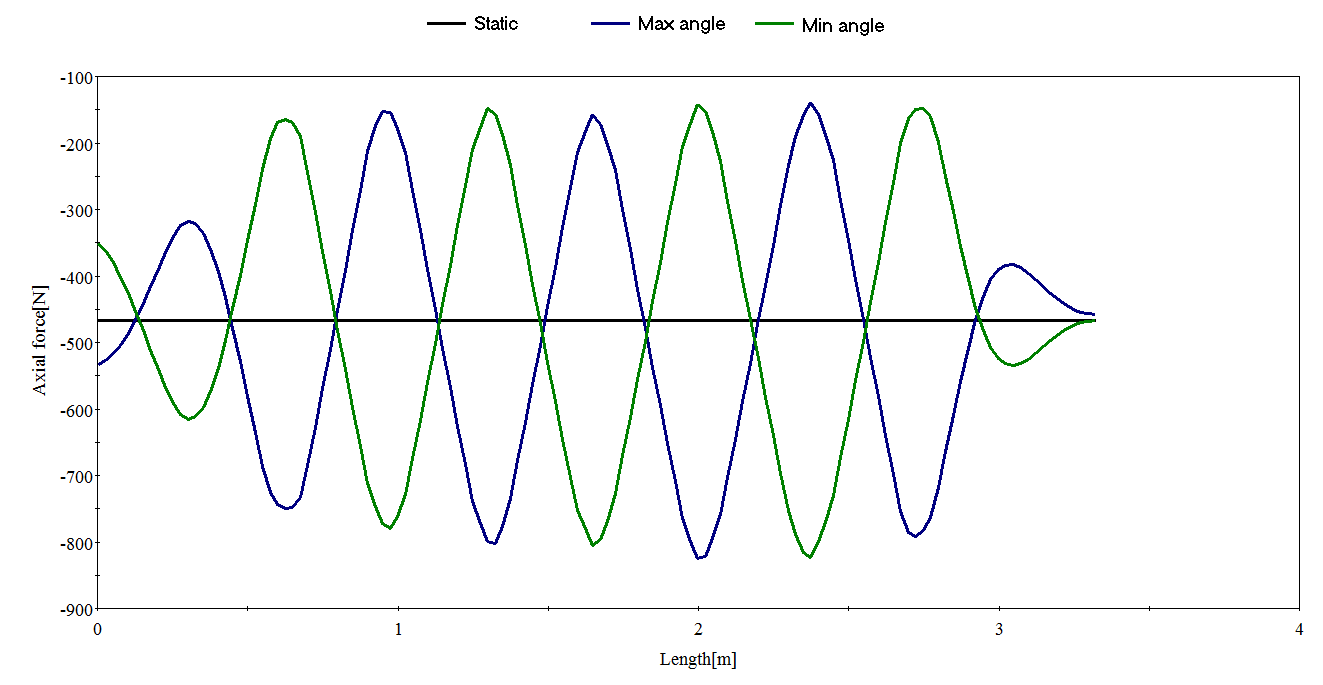
\includegraphics[scale=0.4]{figures/bflexax}
\caption[$\; \:$Axial force in conductors]{Axial force in conductors over length of cable [N]}
 \label{fig:bflexax}
\end{figure}
\noindent Figure \ref{fig:bflexax} shows the axial force distribution over the cable......
\begin{figure}[H]
\centering
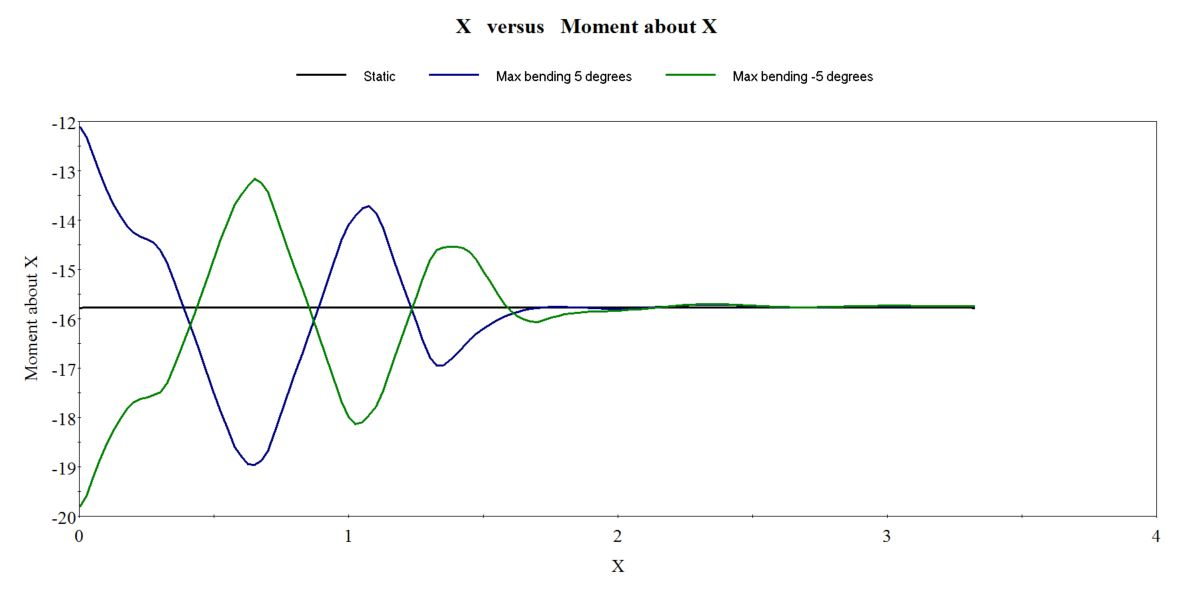
\includegraphics[scale=0.4]{figures/bflexmx}
\caption[$\; \:$Moment about X-Axis in conductors]{Moment about X-Axis in conductors over length of cable  [Nm]}
 \label{fig:bflexmx}
\end{figure}

\begin{figure}[H]
\centering
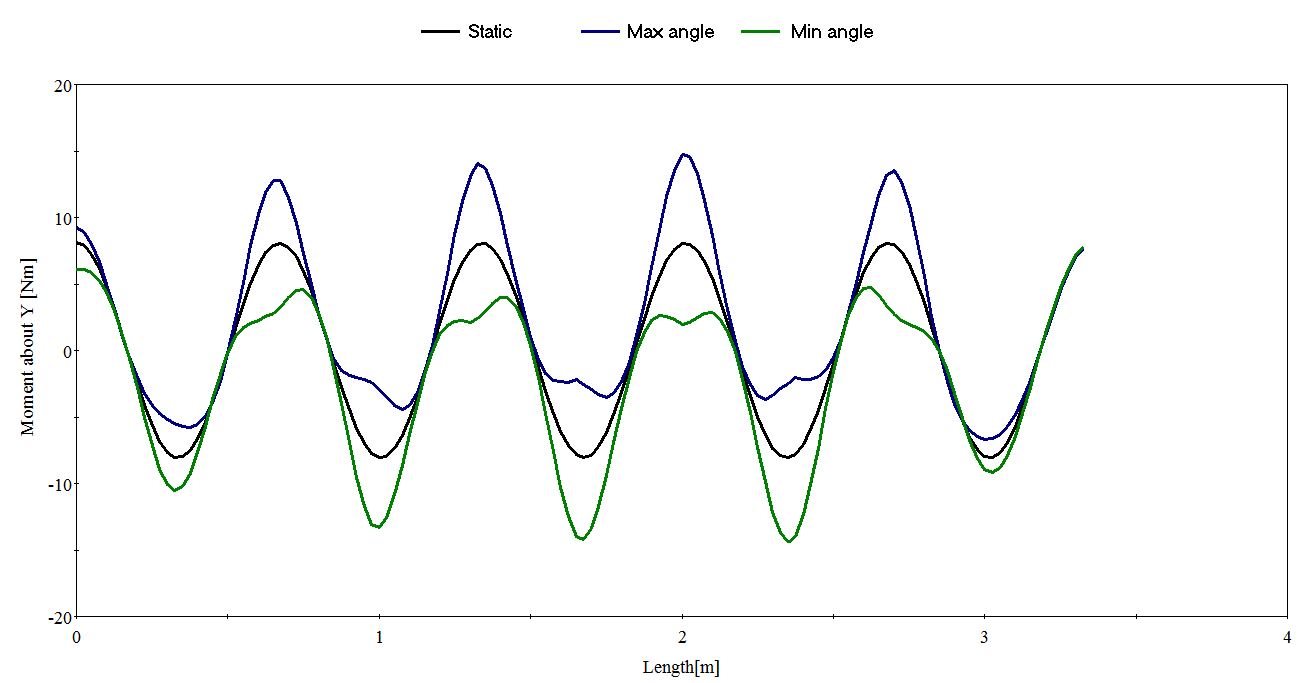
\includegraphics[scale=0.4]{figures/bflexmy}
\caption[$\; \:$Moment about Y-Axis in conductors]{Moment about Y-Axis in conductors over length of cable [Nm]}
 \label{fig:bflexmy}
\end{figure}

\begin{figure}[H]
\centering
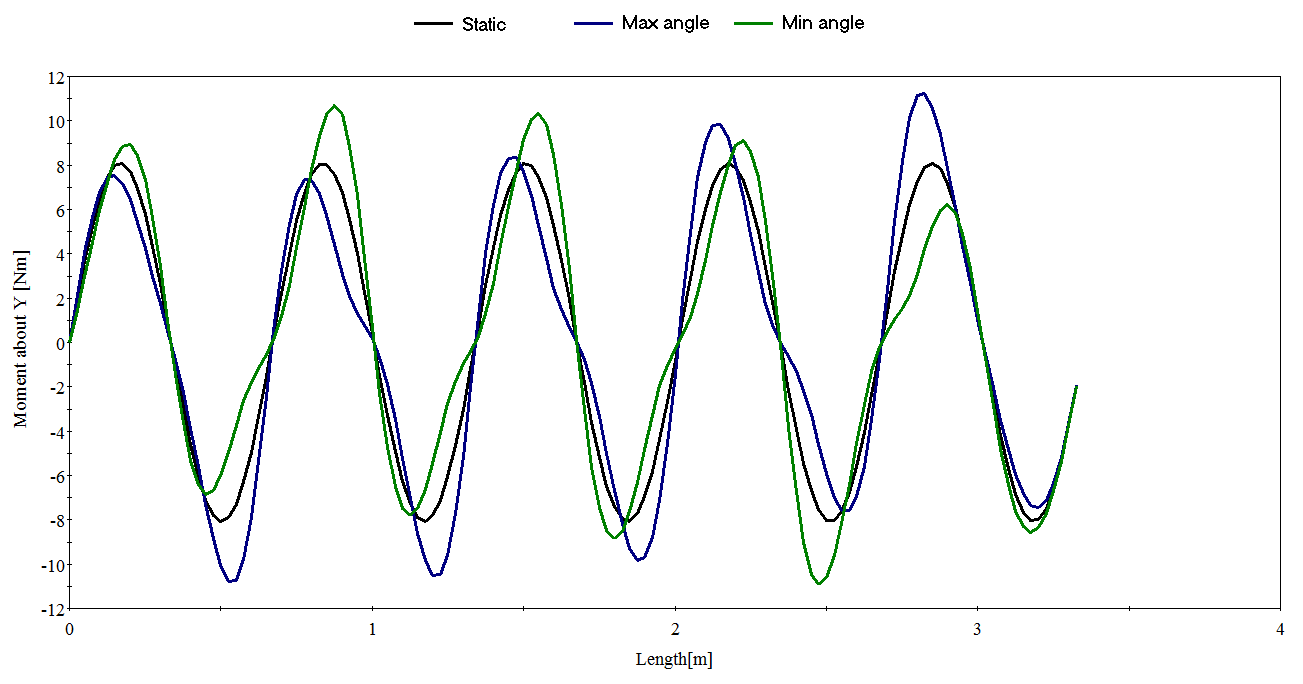
\includegraphics[scale=0.4]{figures/bflexmz}
\caption[$\; \:$Axial force in conductors]{Axial force in conductors over length of cable [Nm]}
 \label{fig:bflexmz}
\end{figure}

\begin{figure}[H]
\centering
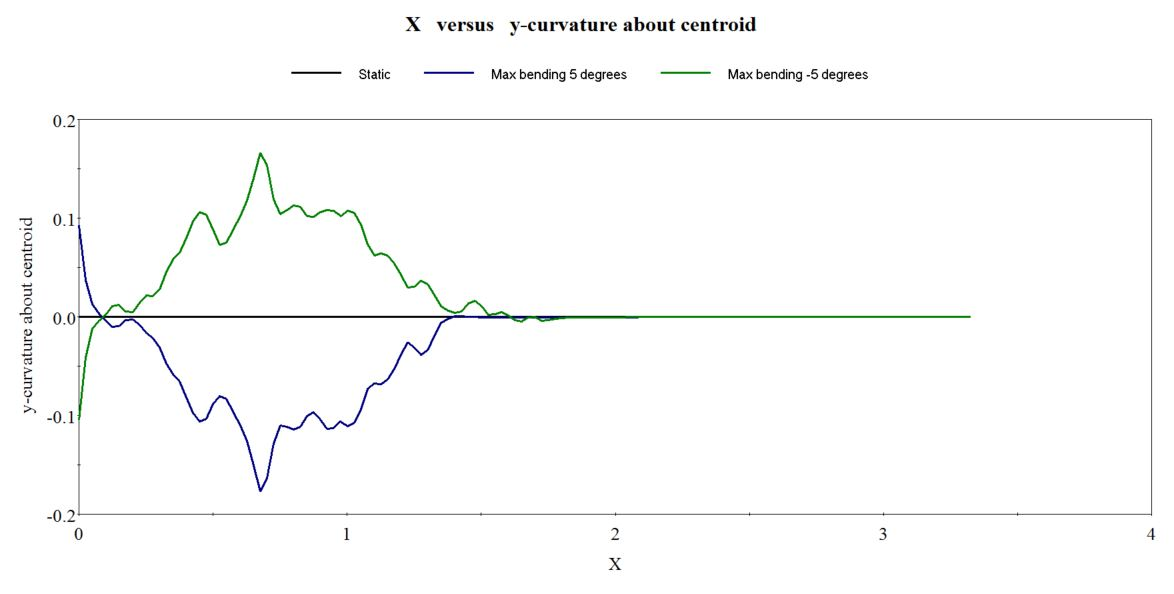
\includegraphics[scale=0.4]{figures/bflexcurve}
\caption[$\; \:$Curvature in outer sheath]{Curvature in the outer sheath over the length of cable [1/m]}
 \label{fig:bflexcurve}
\end{figure}

\section{Bend Stiffener}
\begin{figure}[H]
\centering
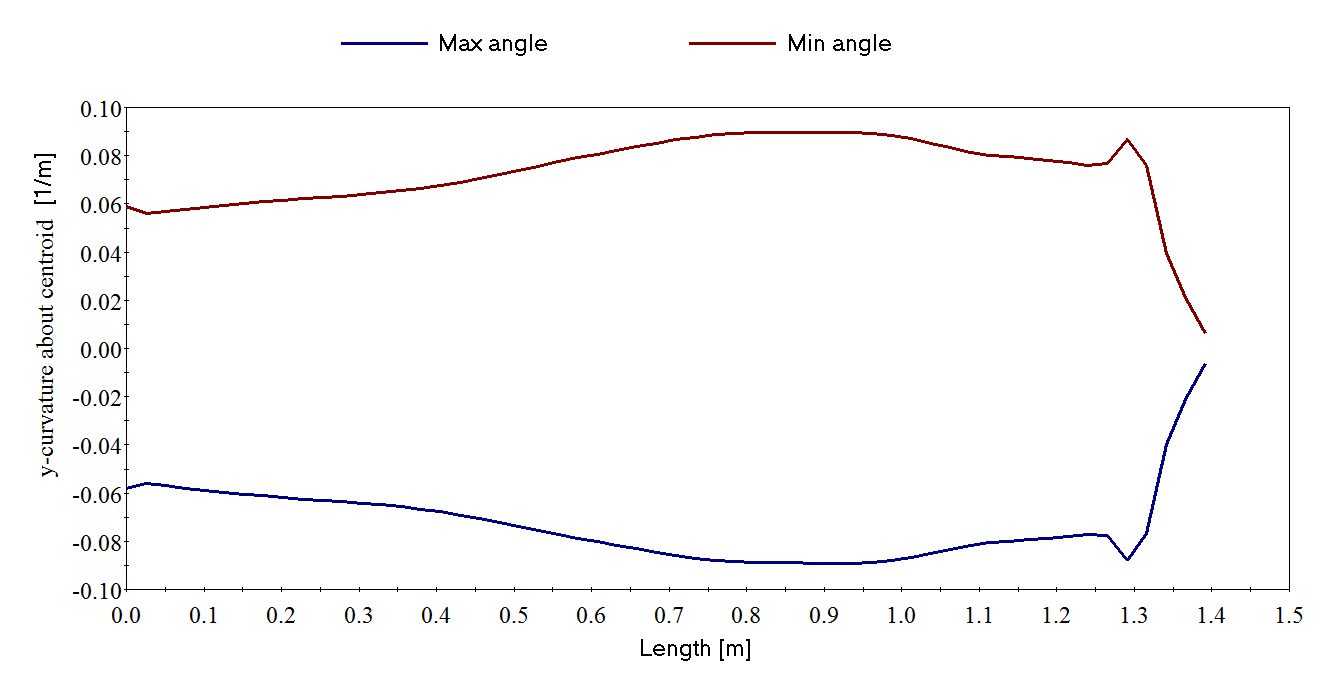
\includegraphics[scale=0.4]{figures/bendstiff}
\caption[$\; \:$Curvature in bend stiffener]{Curvature in bend stiffener}
 \label{fig:bendstiff}
\end{figure}